\chapter{Oscillations}

% ============================================================
\section{The Harmonic Oscillator}
% ============================================================

The prototypical mechanical oscillator is a mass $m$ attached to a spring on a frictionless surface, constrained to move along a single axis. Before we can write down its equation of motion, however, we should be precise about how many numbers we need to specify its state.

\begin{definition}[Degrees of freedom]
The number of \emph{degrees of freedom} (DOF) of a mechanical system is the number of coordinates that must be specified in order to determine its configuration completely.
\end{definition}

For every degree of freedom, Newton's second law will give us a second-order differential equation. Solving the dynamics amounts to solving one such equation of motion per DOF, together with initial conditions. The mass on a spring has a single DOF (Figure~\ref{fig:spring-mass}), so we expect a single second-order ODE governing its motion.

\begin{figure}[ht]
    \centering
    \begin{tikzpicture}[scale=1.0]
        % wall
        \fill[pattern=north east lines] (-0.3,-0.6) rectangle (0,1.0);
        \draw[thick] (0,-0.6) -- (0,1.0);
        % ground
        \draw[thick] (0,-0.6) -- (6,-0.6);
        \fill[pattern=north east lines] (0,-0.8) rectangle (6,-0.6);
        % spring
        \draw[thick, decorate, decoration={coil, aspect=0.6, segment length=5pt, amplitude=5pt}] (0,0.2) -- (3,0.2);
        % mass
        \draw[thick, fill=LightGray] (3,-0.4) rectangle (4.2,0.8);
        \node at (3.6,0.2) {$m$};
        % equilibrium marker and displacement
        \draw[dashed] (3.6,-0.6) -- (3.6,-1.2);
        \node at (3.6,-1.45) {$x_0$};
        \draw[->, thick] (4.2,1.1) -- (5.4,1.1) node[right] {$x$};
    \end{tikzpicture}
    \caption{A mass $m$ on a spring, free to slide along a single axis on a frictionless surface. Its configuration is fixed by one coordinate $x$, so it has a single degree of freedom.}
    \label{fig:spring-mass}
\end{figure}

\subsection{Hooke's Law and the Equation of Motion}

The empirical content of a spring is Hooke's law: the restoring force is proportional to the displacement from the natural length, and directed back toward equilibrium. Writing $x_0$ for the equilibrium position,
\begin{equation}
    F = -k(x - x_0),
\end{equation}
where $k$ is the \emph{spring constant} with units $[k] = MT^{-2}$. Newton's second law then reads
\begin{equation}
    m\ddot{x}(t) = -k\,x(t),
\end{equation}
after shifting coordinates so $x_0 = 0$. Dividing by $m$,
\begin{equation}
    \ddot{x}(t) = -\frac{k}{m}\,x(t).
\end{equation}

This is a second-order linear ODE with constant coefficients. Because the equation asks for a function whose second derivative is proportional to its negative, sines and cosines are natural guesses. We try the ansatz
\begin{equation}
    x(t) = a\cos(\omega t) + b\sin(\omega t),
\end{equation}
whose derivatives are $\dot{x}(t) = -a\omega\sin(\omega t) + b\omega\cos(\omega t)$ and $\ddot{x}(t) = -\omega^2 x(t)$. Substituting back into the equation of motion forces
\begin{equation}
    \omega^2 = \frac{k}{m} \quad\Longrightarrow\quad \omega = \sqrt{\frac{k}{m}}.
\end{equation}

\begin{formula}[Simple harmonic motion]
The mass on a spring obeys
\begin{equation}
    \ddot{x}(t) + \omega^2 x(t) = 0, \qquad \omega \equiv \sqrt{\tfrac{k}{m}},
\end{equation}
whose general solution is $x(t) = a\cos(\omega t) + b\sin(\omega t)$, with $[\omega] = T^{-1}$.
\end{formula}

The quantity $\omega$ is called the \emph{angular frequency}. It is related to the ordinary (cyclic) frequency $f$ by $\omega = 2\pi f$, and the period of oscillation is
\begin{equation}
    T = \frac{2\pi}{\omega}.
\end{equation}
Notice that $\omega$ depends only on the ratio $k/m$: a stiffer spring or a lighter mass yields a faster oscillation, in accord with physical intuition.

\subsection{The Initial Value Problem}

Having obtained the general solution, we now ask what selects a particular trajectory. Since the equation of motion is second-order, its solution has two free constants which are fixed by two initial conditions --- typically the position $x(0)$ and velocity $\dot{x}(0)$. Evaluating the general solution and its derivative at $t=0$ gives $a = x(0)$ and $b = \dot{x}(0)/\omega$, so
\begin{formula}
\begin{equation}
    x(t) = x(0)\cos(\omega t) + \frac{\dot{x}(0)}{\omega}\sin(\omega t).
\end{equation}
\end{formula}

\begin{fact}[Uniqueness of solutions]
Solutions of a linear second-order ODE are unique given a choice of initial conditions: exactly one trajectory passes through a specified $(x(0), \dot{x}(0))$.
\end{fact}

Uniqueness is a strong statement: two harmonic oscillators started with the same position and velocity will trace out identical trajectories forever after, no matter how similar or different their pasts.

\subsection{The Simple Harmonic Oscillator in General Coordinates}

Our derivation quietly assumed we could shift coordinates so that equilibrium sits at the origin. It is worth confirming that nothing depends on this choice. If the spring's natural length is $\ell_0$ and the mass is at position $x$, define the displacement from equilibrium $\Delta x \equiv x - \ell_0$. Since $\ell_0$ is constant, $\dot{\Delta x} = \dot{x}$ and $\ddot{\Delta x} = \ddot{x}$, so Hooke's law and Newton's law together read
\begin{equation}
    F = -k\,\Delta x, \qquad m\,\ddot{\Delta x} = -k\,\Delta x,
\end{equation}
which has exactly the same form as before. This is our first hint that the essential content of ``simple harmonic motion'' is really the \emph{form} of the equation, not the particular coordinate we use --- a theme that will recur when we meet pendula, LC circuits, and other systems that share the same underlying equation.

\subsection{Assumptions of the Spring--Mass System}

The clean SHM equation we derived rests on a handful of idealizations. We have assumed that the spring is ideal and obeys Hooke's law exactly, that there is no friction, that motion is confined to a single axis, that the initial conditions are known perfectly, and that the setup is in an inertial frame. Each of these can be relaxed --- introducing damping, driving forces, coupled coordinates, or noninertial effects --- and each relaxation gives rise to a richer class of phenomena that we will meet in later chapters. For now the point is that even the ``simple'' oscillator is a controlled idealization of a much messier reality.

% ============================================================
\section{Small Oscillations and Linearity}
% ============================================================

We turn now from this single example to the broad structural reason it appears so often in physics. The equation of motion for the harmonic oscillator is a special case of a much broader class of \emph{linear} equations, and it is linearity that underwrites almost every technique we will use.

\subsection{Linear Systems}

\begin{definition}[Linear system, 1 DOF]
A one-degree-of-freedom system is \emph{linear} if its equation of motion is a linear function of the coordinate $x$ and its derivatives, taking the form
\begin{equation}
    \alpha\,\ddot{x}(t) + \beta\,\dot{x}(t) + \gamma\,x(t) = f(t), \label{eq:linear-ode}
\end{equation}
where no derivative higher than the second appears. The system is \emph{homogeneous} if every term contains exactly one power of $x$ (or its derivatives), i.e.\ if $f(t) = 0$.
\end{definition}

The great virtue of linear equations is the \emph{superposition principle}. Suppose $x_1$ and $x_2$ are two solutions of the inhomogeneous equation with forcings $f_1$ and $f_2$:
\begin{align}
    \alpha\ddot{x}_1 + \beta\dot{x}_1 + \gamma x_1 &= f_1(t), \\
    \alpha\ddot{x}_2 + \beta\dot{x}_2 + \gamma x_2 &= f_2(t).
\end{align}
Adding these equations, linearity of differentiation gives
\begin{equation}
    \alpha(\ddot{x}_1 + \ddot{x}_2) + \beta(\dot{x}_1 + \dot{x}_2) + \gamma(x_1 + x_2) = f_1(t) + f_2(t),
\end{equation}
so $x_1 + x_2$ is a solution with forcing $f_1 + f_2$. More generally, \emph{any} linear combination $A x_1 + B x_2$ of two homogeneous solutions is again a homogeneous solution. In other words, the homogeneous solution space is a vector space, and we may attack any solution by decomposing it into simpler pieces.

\begin{theorem}[General solution of a linear ODE]
The general solution of a linear inhomogeneous equation is the sum of the general homogeneous solution and any particular solution of the inhomogeneous equation:
\begin{equation}
    x(t) = x_h(t) + x_p(t).
\end{equation}
\end{theorem}

\subsection{Different Ways to Write the Solution}

Superposition guarantees that the homogeneous SHM solution can be written in several equivalent representations, each convenient in a different context:
\begin{align}
    x(t) &= A\cos(\omega t) + B\sin(\omega t), \\
    x(t) &= A\cos(\omega t + \phi), \\
    x(t) &= \operatorname{Re}\!\left\{A\,e^{i(\omega t + \phi)}\right\}, \\
    x(t) &= \operatorname{Re}\!\left\{A\,e^{i\omega t} + B\,e^{-i\omega t}\right\}.
\end{align}
The first uses two real amplitudes and is closest to what the initial-value problem produces directly; the second replaces them with an amplitude and phase, which is what an experimentalist actually measures; the last two use complex exponentials, which will prove indispensable once we discuss time-translation invariance. The following example shows how easily one passes between these forms.

\begin{example}[Rewriting a phase-shifted exponential]
Let $x(t) = \operatorname{Re}\{A e^{-i(\omega t + \pi/2)}\}$. Factoring the phase,
\begin{equation}
    A e^{-i(\omega t + \pi/2)} = A e^{-i\pi/2} e^{-i\omega t} = -iA\,(\cos\omega t - i\sin\omega t) = -A\sin\omega t - iA\cos\omega t,
\end{equation}
so $\operatorname{Re}\{x(t)\} = -A\sin(\omega t)$. A phase shift of $-\pi/2$ has converted a cosine into a (negative) sine, illustrating how the phase in the complex form encodes the mixture of $\cos$ and $\sin$ in the real form.
\end{example}

\subsection{Linearity in Nature: Small Oscillations}

Real physical systems are almost never exactly linear. What justifies studying linear equations so intensively? The answer is that near a stable equilibrium, \emph{almost every} conservative system behaves linearly to leading order.

Consider a particle of position $x$ moving in a potential $V(x)$. For a conservative force,
\begin{equation}
    F(x) = -\dv{V}{x}.
\end{equation}
Equilibria are points where $F = 0$, i.e.\ where $V'(x) = 0$. Choose coordinates so that $x_0 = 0$ is such an equilibrium and Taylor expand:
\begin{equation}
    F(x) = -V'(x) = -V'(0) - V''(0)\,x - \tfrac{1}{2} x^2 V'''(0) - \cdots
\end{equation}
The first term vanishes because $x_0 = 0$ is an equilibrium. If we keep only the linear term, we get Hooke's law with effective spring constant $k = V''(0)$, and the motion is simple harmonic. The higher-order terms are negligible provided
\begin{equation}
    |x\,V'''(0)| \ll V''(0),
\end{equation}
which sets a length scale $L$ such that the linear approximation is valid for $|x| \ll L$.

\begin{fact}[Conditions for approximate linearity to fail]
A conservative force near equilibrium fails to be approximately linear if either the potential is not well-defined at equilibrium, or $V''(0) = 0$ so that the leading nonvanishing term in the expansion is cubic or higher. (In the latter case, stability additionally forces $V'''(0) = 0$, so the leading nontrivial term is quartic.)
\end{fact}

\subsection{Example: A Nontrivial Potential}

To see the general lesson at work, consider the potential
\begin{equation}
    V(x) = E\!\left(\frac{L}{x} + \frac{x}{L}\right).
\end{equation}
Its derivative is
\begin{equation}
    V'(x) = -\frac{EL}{x^2} + \frac{E}{L} = E\!\left(\frac{1}{L} - \frac{L}{x^2}\right),
\end{equation}
which vanishes when $x = \pm L$. Choose the positive root and change variables to the displacement $y = x - L$, so that $y = 0$ marks the equilibrium. The force in the new coordinate is
\begin{equation}
    F(y) = -V'(y+L) = E\!\left(\frac{L}{(y+L)^2} - \frac{1}{y+L}\right).
\end{equation}
Its derivatives are
\begin{equation}
    F'(y) = \frac{-2EL}{(y+L)^3}, \quad F'(0) = -\frac{2E}{L^2}, \qquad
    F''(y) = \frac{6EL}{(y+L)^4}, \quad F''(0) = \frac{6E}{L^3},
\end{equation}
so
\begin{equation}
    F(y) \approx -\frac{2E}{L^2}\,y + \frac{3E}{L^3}\,y^2 + \cdots.
\end{equation}
The ratio of the quadratic correction to the linear term is
\begin{equation}
    \frac{3E y^2 / L^3}{2E y / L^2} = \frac{3y}{2L},
\end{equation}
which is small precisely when $|y| \ll L$, confirming the general lesson: linearity is a good approximation for displacements small compared with the natural length scale of the potential. Figure~\ref{fig:small-osc} shows this potential together with the parabola that approximates it near the minimum; the two agree closely in a neighborhood of equilibrium and part ways only once the displacement becomes comparable to $L$.

\begin{figure}[ht]
    \centering
    \begin{tikzpicture}
    \begin{axis}[
        width=10cm, height=6.2cm,
        xlabel=$x/L$, ylabel=$V/E$,
        domain=0.3:3.0, samples=200,
        xmin=0, xmax=3, ymin=1.8, ymax=4.2,
        axis lines=left, xtick={1}, xticklabels={$L$}, ytick={2}, yticklabels={$2E$},
        legend pos=north east, legend cell align=left,
        every axis plot/.append style={thick},
    ]
        \addplot[Periwinkle] {x + 1/x};
        \addlegendentry{$V(x)=E\left(\tfrac{L}{x}+\tfrac{x}{L}\right)$}
        \addplot[Orange, dashed, domain=0.4:1.6] {2 + (x-1)^2};
        \addlegendentry{parabolic approximation}
        \addplot[gray, dotted, samples=2, domain=0:3] coordinates {(1,1.8) (1,2)};
    \end{axis}
    \end{tikzpicture}
    \caption{Near a stable equilibrium every smooth potential looks parabolic. The potential $V(x)=E(L/x+x/L)$ (solid) and its quadratic approximation $2E + (E/L^2)(x-L)^2$ (dashed) agree for $|x-L|\ll L$, which is exactly the regime of simple harmonic motion.}
    \label{fig:small-osc}
\end{figure}

\begin{example}[Equilibria of a quartic potential]
Consider $V(x) = (V_0/a^4)(x^4 + 4ax^3 - 8a^2 x^2)$ with $a > 0$. Solving $V'(x) = (V_0/a^4)(4x^3 + 12ax^2 - 16a^2 x) = 0$ gives $x = 0, a, -4a$. Computing $V''(x) = (4V_0/a^4)(3x^2 + 6ax - 4a^2)$: at $x=0$ we get $V''(0) = -16V_0/a^2 < 0$ (unstable maximum), while at $x = a$ and $x = -4a$ we get $V''(a) = 20V_0/a^2 > 0$ and $V''(-4a) = 80V_0/a^2 > 0$, both stable. Small oscillations about $x = a$ therefore obey $m\ddot{y} = -V''(a)\,y$ with $y = x - a$, giving angular frequency $\omega = \sqrt{20 V_0/(m a^2)}$. This illustrates the whole procedure: locate equilibria, discard the unstable ones, and read off the local Hooke constant from $V''$.
\end{example}

\subsection{Example: The Solid Pendulum}

A second application of the same idea: take a uniform rod of length $\ell$ and mass $m$ pivoted about one end, so that its moment of inertia about the pivot is $I = m\ell^2/3$. Let $\theta$ be the angle from the downward vertical. The gravitational force acts at the center of mass, a distance $\ell/2$ from the pivot, and produces a torque
\begin{equation}
    \tau = |\vect{r}\times\vect{F}| = -mg\,\tfrac{\ell}{2}\sin\theta.
\end{equation}
Newton's law for rotational motion, $\tau = I\ddot{\theta}$, gives
\begin{equation}
    \frac{m\ell^2}{3}\,\ddot{\theta} = -\frac{mg\ell}{2}\sin\theta \quad\Longrightarrow\quad \ddot{\theta}(t) = -\frac{3g}{2\ell}\sin\theta(t).
\end{equation}
The exact equation is nonlinear because of the $\sin\theta$, but for small angles $\sin\theta \approx \theta$ and it linearizes to
\begin{equation}
    \ddot{\theta}(t) \approx -\frac{3g}{2\ell}\,\theta(t),
\end{equation}
which is simple harmonic motion with angular frequency $\omega = \sqrt{3g/(2\ell)}$. Once again a physically nonlinear system yields SHM in the small-oscillation limit.

% ============================================================
\section{Time Translation Invariance}
% ============================================================

Having established that linearity is generic, we now identify a second structural feature of oscillator equations --- one that will single out the exponential functions as the natural basis of solutions. Return to the homogeneous linear equation
\begin{equation}
    \alpha\,\ddot{x}(t) + \beta\,\dot{x}(t) + \gamma\,x(t) = 0. \label{eq:homog}
\end{equation}
Because the coefficients $\alpha, \beta, \gamma$ do not depend on $t$, the equation looks the same at every instant of time. This symmetry has a powerful consequence.

\begin{fact}[Time-translation invariance]
If $x(t)$ is a solution of a homogeneous linear ODE with constant coefficients, then $x(t + a)$ is also a solution, for any constant $a \in \mathbb{R}$.
\end{fact}

Intuitively, this is because $\dv{}{t}$ acts identically on functions of $t$ and functions of $t + a$: the differential operator commutes with shifts.

Working directly with expressions like $x(t + a)$ is cumbersome, however. The natural bookkeeping device is complex exponentials, which convert time shifts into multiplication: $e^{i\omega(t+a)} = e^{i\omega a}\,e^{i\omega t}$. This motivates the whole apparatus of complex-number methods for oscillations, to which we turn shortly.

\subsection{Connection with Uniform Circular Motion}

A hint that SHM is deeply tied to rotation comes from projecting uniform circular motion onto an axis. A particle moving on a circle of radius $R$ with angular speed $\omega$ has Cartesian coordinates
\begin{equation}
    x(t) = R\cos(\omega t - \phi), \qquad y(t) = -R\sin(\omega t - \phi).
\end{equation}
At $t = 0$,
\begin{equation}
    x(0) = R\cos\phi, \qquad \dot{x}(0) = \omega R\sin\phi,
\end{equation}
and $x(t)$ satisfies exactly the SHM equation $\ddot{x} = -\omega^2 x$. Simple harmonic motion is nothing but the shadow of uniform circular motion (Figure~\ref{fig:circular-shadow}) --- and it is precisely this rotational picture that complex exponentials will make algebraically transparent.

\begin{figure}[ht]
    \centering
    \begin{tikzpicture}[scale=1.6]
        % axes
        \draw[->] (-1.4,0) -- (1.6,0) node[right] {$x$};
        \draw[->] (0,-1.4) -- (0,1.5) node[above] {$y$};
        % circle
        \draw[thick, Periwinkle] (0,0) circle (1);
        % angle
        \def\ang{55}
        \coordinate (P) at (\ang:1);
        \draw[thick, -{Stealth}] (0,0) -- (P);
        \draw (0.35,0) arc (0:\ang:0.35);
        \node at (0.55,0.25) {$\omega t$};
        % point
        \fill (P) circle (1.2pt);
        \node[above right] at (P) {};
        % projection onto x-axis
        \draw[dashed] (P) -- (\ang:1 |- 0,0);
        \fill[Orange] (\ang:1 |- 0,0) circle (1.2pt);
        \draw[->, Orange, thick] (0,-0.15) -- ($({cos(\ang)},0)+(0,-0.15)$);
        \node[Orange, below] at (0.3,-0.2) {$x=R\cos\omega t$};
        \node[right] at (1.02,-0.02) {$R$};
    \end{tikzpicture}
    \caption{A particle in uniform circular motion at angular speed $\omega$; its projection onto the $x$-axis executes simple harmonic motion $x(t)=R\cos\omega t$. The shadow oscillates while the particle merely rotates.}
    \label{fig:circular-shadow}
\end{figure}

% ============================================================
\section{Complex Numbers}
% ============================================================

The natural language for time-translation-invariant dynamics is complex analysis. We collect the essentials here.

\begin{formula}[Euler's identity]
\begin{equation}
    e^{i\theta} = \cos\theta + i\sin\theta.
\end{equation}
\end{formula}

For $z = a + ib$, the real and imaginary parts can be recovered from $z$ and its complex conjugate $z^* = a - ib$ via
\begin{equation}
    \operatorname{Re}(z) = \frac{z + z^*}{2}, \qquad \operatorname{Im}(z) = \frac{z - z^*}{2i}.
\end{equation}

\subsection{Modulus and Argument}

The absolute value of $z = a + ib$ is
\begin{equation}
    |z| = \sqrt{a^2 + b^2} = \sqrt{z z^*},
\end{equation}
and behaves multiplicatively under products and quotients:
\begin{equation}
    |z z'| = |z||z'|, \qquad \left|\tfrac{z}{z'}\right| = \frac{|z|}{|z'|}.
\end{equation}
The \emph{argument} is the angle $z$ makes with the positive real axis:
\begin{equation}
    \arg(z) = \begin{cases} \tan^{-1}(b/a), & a \geq 0, \\ \tan^{-1}(b/a) + \pi, & a < 0. \end{cases}
\end{equation}
The extra $\pi$ in the second and third quadrants corrects for the fact that $\tan^{-1}$ only returns angles in $(-\pi/2, \pi/2)$.

In polar form, any complex number $z = x + iy$ can be written
\begin{equation}
    z = R e^{i\theta}, \qquad R = |z|, \qquad \theta = \arg(z).
\end{equation}

\subsection{Complex Exponential Identities}

Inverting Euler's identity gives compact expressions for the trigonometric functions:
\begin{formula}
\begin{equation}
    \cos\theta = \frac{e^{i\theta} + e^{-i\theta}}{2}, \qquad \sin\theta = \frac{e^{i\theta} - e^{-i\theta}}{2i}.
\end{equation}
\end{formula}
Multiple-angle identities follow effortlessly: for instance $\cos(3\theta) = \operatorname{Re}\{e^{3i\theta}\} = \operatorname{Re}\{(\cos\theta + i\sin\theta)^3\}$ expands via the binomial theorem.

A useful sum-to-product identity, obtained by adding $\cos(\theta+\theta')$ and $\cos(\theta-\theta')$:
\begin{equation}
    \cos(\theta+\theta') + \cos(\theta-\theta') = 2\cos\theta\cos\theta'.
\end{equation}

% ============================================================
\section{Exponential Solutions}
% ============================================================

We now put linearity and time-translation invariance together to solve second-order linear ODEs systematically. Consider the mass--spring equation, but allow the solution to be complex-valued:
\begin{equation}
    M\,\ddot{z}(t) + K\,z(t) = 0, \qquad z(t) : \mathbb{R} \to \mathbb{C}.
\end{equation}
Since $i$ is a constant and the ODE is linear with real coefficients, if $z(t)$ solves the equation then so do $\operatorname{Re}\{z\}$ and $\operatorname{Im}\{z\}$ individually. Complex solutions are thus a convenient bookkeeping device that packages two real solutions at once.

\subsection{Why Complex Exponentials?}

We claim that time-translation invariance forces the fundamental solutions to be exponentials. The argument rests on two ingredients. First, \emph{linearity} tells us that the solution space of a homogeneous linear $n$th-order ODE is $n$-dimensional; picking a basis $x_1(t), \ldots, x_n(t)$ we can write any solution as $z(t) = \sum_j c_j x_j(t)$. Second, \emph{time-translation invariance} lets us look for solutions on which time shifts act particularly simply --- by scalar multiplication:
\begin{equation}
    z(t + a) = h(a)\,z(t), \label{eq:tt-eigen}
\end{equation}
for some scalar function $h(a)$.

Since each basis function $x_j(t + a)$ must itself be a linear combination of the basis, we have
\begin{equation}
    x_j(t + a) = \sum_k R_{jk}(a)\,x_k(t),
\end{equation}
for some matrix $R(a)$. Plugging into~\eqref{eq:tt-eigen} yields an eigenvalue equation for the coefficient vector $\vect{c}$:
\begin{equation}
    R(a)\,\vect{c} = h(a)\,\vect{c}, \qquad (R(a) - h(a)\,\mathbb{1})\vect{c} = 0.
\end{equation}
Setting $\det(R(a) - h(a)\mathbb{1}) = 0$ gives (at most) $n$ complex values of $h(a)$, one for each independent exponential mode.

\subsection{The Exponential Form}

To find the form of these ``irreducible'' solutions, differentiate~\eqref{eq:tt-eigen} with respect to $a$ and set $a = 0$:
\begin{equation}
    z'(t) = H\,z(t), \qquad H \equiv h'(0),
\end{equation}
whose solution is $z(t) \propto e^{Ht}$.

An alternative derivation: set $t = 0$ in $z(t + a) = h(a)z(t)$ to get $h(a) = z(a)/z(0)$. Normalizing $z(0) = 1$ gives $h(a) = z(a)$, so
\begin{equation}
    z(t + a) = z(t)\,z(a).
\end{equation}
For small $\varepsilon$, Taylor expansion yields $z(\varepsilon) \approx 1 + H\varepsilon + O(\varepsilon^2)$, and iterating,
\begin{equation}
    z(t) = \lim_{N\to\infty}\left[z(t/N)\right]^N = \lim_{N\to\infty}\left[1 + H(t/N)\right]^N = e^{Ht}.
\end{equation}

\begin{formula}[Exponential ansatz]
Linear ODEs with constant coefficients admit complex-exponential solutions:
\begin{equation}
    z(t) = e^{Ht},
\end{equation}
for some (generally complex) constant $H$ determined by the equation.
\end{formula}

\subsection{Applying to the Mass--Spring Equation}

Substituting $z(t) = e^{Ht}$ into $M\ddot{z} + K z = 0$:
\begin{equation}
    (M H^2 + K)\,e^{Ht} = 0 \quad\Longrightarrow\quad M H^2 + K = 0.
\end{equation}
So $H^2 = -K/M$, giving
\begin{equation}
    H = \pm i\omega, \qquad \omega \equiv \sqrt{\tfrac{K}{M}}.
\end{equation}
The two independent complex solutions are
\begin{equation}
    z(t) = e^{\pm i\omega t},
\end{equation}
whose real and imaginary parts are $\cos(\omega t)$ and $\pm\sin(\omega t)$, recovering the sinusoidal solutions we found before. The exponential ansatz has thus reproduced our earlier ad-hoc guess, but with a principled justification that generalizes to damped and driven systems.

\subsection{Amplitude and Phase Form}

Given any real solution $x(t) = c\cos(\omega t) + d\sin(\omega t)$, we can rewrite it in \emph{amplitude-phase form}. Using the complex exponential identities,
\begin{align}
    c\cos(\omega t) + d\sin(\omega t) &= \frac{c}{2}(e^{i\omega t} + e^{-i\omega t}) - \frac{id}{2}(e^{i\omega t} - e^{-i\omega t}) \\
    &= \operatorname{Re}\!\left\{(c + id)\,e^{-i\omega t}\right\} \\
    &= \operatorname{Re}\!\left\{A\,e^{i\theta}\,e^{-i\omega t}\right\} = A\cos(\omega t - \theta),
\end{align}
where
\begin{formula}
\begin{equation}
    A = \sqrt{c^2 + d^2}, \qquad \theta = \arg(c + id).
\end{equation}
\end{formula}
By convention we work with solutions of the form $z(t) = A\,e^{-i(\omega t - \theta)}$; the physical displacement is its real part.

\begin{example}[Two-spring oscillator]
A mass $m$ is attached between a wall on the left by a spring of constant $K$ and a wall on the right by a spring of constant $2K$, both initially at their natural lengths. Let $\Delta x$ be the mass's displacement from equilibrium. The left spring pulls with force $-K\Delta x$ and the right spring pushes with force $-2K\Delta x$, so
\begin{equation}
    m\,\ddot{\Delta x} = -3K\,\Delta x, \qquad \omega = \sqrt{\tfrac{3K}{m}}.
\end{equation}
If the mass starts at rest at equilibrium and is given velocity $V$, then $\Delta x(0) = 0$ and $\dot{\Delta x}(0) = V$, so the general solution $\Delta x(t) = a\cos\omega t + b\sin\omega t$ reduces to
\begin{equation}
    \Delta x(t) = \frac{V}{\omega}\sin(\omega t) = V\sqrt{\frac{m}{3K}}\,\sin\!\left(\sqrt{\tfrac{3K}{m}}\,t\right).
\end{equation}
In complex form, using $\sin\omega t = \operatorname{Re}\{-i e^{i\omega t}\} = \operatorname{Re}\{e^{i(\omega t - \pi/2)}\}$, this is $\Delta x(t) = \operatorname{Re}\{(V/\omega)\,e^{i(\omega t - \pi/2)}\}$: springs in parallel add their constants, and the initial condition ``pure velocity'' selects a $-\pi/2$ phase.
\end{example}
% ============================================================
\section{Damped Oscillators (Preview)}
% ============================================================
Adding a velocity-dependent damping term $\Gamma\dot{x}$ to the equation of motion produces the \emph{damped harmonic oscillator}:
\begin{equation}
    \ddot{x} + \Gamma\dot{x} + \omega_0^2\,x = 0.
\end{equation}
Here the three physical terms are the \emph{inertial} term $\ddot{x}$, the \emph{damping} term $\Gamma\dot{x}$, and the \emph{restoring force} $\omega_0^2 x$. The exponential ansatz $x(t) = e^{Ht}$ gives a quadratic $H^2 + \Gamma H + \omega_0^2 = 0$ whose solutions are $H = -\Gamma/2 \pm i\omega$ with
\begin{equation}
    \omega = \sqrt{\omega_0^2 - \tfrac{\Gamma^2}{4}}.
\end{equation}
The character of the motion depends on the sign of the quantity under the square root. When the restoring force dominates ($\omega_0 > \Gamma/2$), $\omega$ is real and the system is \emph{underdamped}: it oscillates at the reduced frequency $\omega$ while its amplitude decays exponentially. When damping dominates ($\omega_0 < \Gamma/2$), $\omega$ is imaginary and the system is \emph{overdamped}: both roots for $H$ are real and negative, so the motion is a pure exponential decay with no oscillation. The boundary case $\omega_0 = \Gamma/2$ is \emph{critical damping}, where $\omega = 0$ and the system returns to equilibrium as fast as possible without overshooting. In the underdamped case one finds
\begin{equation}
    x(t) = A\,e^{-\Gamma t / 2}\cos(\omega t + \phi),
\end{equation}
whose two free parameters $A$ and $\phi$ are fixed by two initial conditions. A more thorough treatment appears in the next chapter.

% ============================================================
\section{LC Circuits, Displacement, and Energy}
% ============================================================

\subsection{The LC Circuit as a Harmonic Oscillator}

The mechanical oscillator has a beautiful electrical analog. In a series circuit containing an inductor $L$ and a capacitor $C$, Faraday's law gives the voltage across the inductor
\begin{equation}
    \Delta V_L = \varepsilon = -L\,\dv{I}{t} = -L\,\dv[2]{Q}{t},
\end{equation}
using $I = \dot{Q}$. Across the capacitor,
\begin{equation}
    \Delta V_C = \frac{Q(t)}{C}.
\end{equation}
Kirchhoff's loop rule says the sum of the voltage drops around the loop is zero, so
\begin{equation}
    \frac{Q(t)}{C} = -L\,\dv[2]{Q}{t} \quad\Longrightarrow\quad L\ddot{Q} + \frac{Q}{C} = 0.
\end{equation}
This is precisely the form of the mass--spring equation $m\ddot{x} + kx = 0$.

\begin{formula}[Mechanical--electrical analogy]
\begin{equation}
    k \longleftrightarrow \frac{1}{C}, \qquad Q \longleftrightarrow x, \qquad L \longleftrightarrow m.
\end{equation}
The charge on the capacitor oscillates sinusoidally at angular frequency $\omega = 1/\sqrt{LC}$.
\end{formula}

\subsection{Generalized Harmonic Oscillator}

The lesson is that ``the'' harmonic oscillator is not really about masses or springs but about any pair of quantities coupled by an equation of the canonical form:
\begin{equation}
    M\,\dv[2]{X}{t} = -K\,X.
\end{equation}
Here $X$ is a \emph{generalized coordinate} (position, charge, angle, \ldots), $M$ is a \emph{generalized mass} (inertia, inductance, moment of inertia), and $K$ is a \emph{generalized spring constant} (Hooke constant, inverse capacitance, torsion constant).

\subsection{Generalized Energy}

Whatever the interpretation, the combination
\begin{equation}
    E = \tfrac{1}{2}M\dot{X}^2 + \tfrac{1}{2}K X^2
\end{equation}
must carry units of energy (joules). As a consistency check for the LC circuit,
\begin{equation}
    [K] = \left[\tfrac{1}{C}\right] = \frac{\text{volts}}{\text{coulombs}} = \frac{\text{joules}}{\text{coulombs}^2},
\end{equation}
so $\tfrac{1}{2}(1/C)Q^2$ has units of joules, as it should.

\subsection{Energy Conservation for the Undriven Oscillator}

Consider the standard sinusoidal solution
\begin{equation}
    X(t) = A\sin(\omega t), \qquad \dot{X}(t) = A\omega\cos(\omega t).
\end{equation}
For a homogeneous linear system (no external driving force, RHS of the ODE equals zero), the oscillator equation gives $K = \omega^2 M$. Substituting into the energy,
\begin{align}
    E(t) &= \tfrac{1}{2}M(A\omega\cos(\omega t))^2 + \tfrac{1}{2}\omega^2 M (A\sin(\omega t))^2 \\
    &= \tfrac{1}{2}M\omega^2 A^2\cos^2(\omega t) + \tfrac{1}{2}M\omega^2 A^2\sin^2(\omega t) \\
    &= \tfrac{1}{2}M\omega^2 A^2 = \tfrac{1}{2}K A^2.
\end{align}
The total energy is constant in time --- kinetic and potential energies exchange sinusoidally, but their sum is conserved. This is the hallmark of undamped harmonic motion.
